\documentclass[11pt,twoside]{article}
\usepackage[T1]{fontenc}
\usepackage[latin1]{inputenc}
\usepackage[english]{babel}
\usepackage{times}
\usepackage{amsmath}
\usepackage{amssymb}
\usepackage{amsthm}
\usepackage{listings}
\usepackage{url}
\usepackage{hyperref}
\usepackage{graphicx}
\usepackage{multirow}
\usepackage{tabularx}
\usepackage{fancyhdr}
\usepackage{lastpage}
\usepackage{listings}
\usepackage{tikz} 
\usepackage[a4paper,margin=2.5cm,hmarginratio=1:1]{geometry}
\usepackage{biblatex} %Imports biblatex package
\usetikzlibrary{graphs}

\addbibresource{references.bib} %Import the bibliography file

%%%%%%%%%%%%%%%%%%%%%%%%%%%%%%%%%%%%%%%%%%%%%%%%%%%%%%%%%%%%%%%%%%%%%%%%%%%
%%%%%%%%%%%%%% ENTER YOUR PERSONAL INFORMATION HERE %%%%%%%%%%%%%%%%%%%%%%%
%%%%%%%%%%%%%%%%%%%%%%%%%%%%%%%%%%%%%%%%%%%%%%%%%%%%%%%%%%%%%%%%%%%%%%%%%%%

% The info of your group members. Set Y and Z empty if you are not
% three.

% THIS FIRST ONE IS YOU.
\newcommand{\persnrX}{0123455789}
\newcommand{\nameX}{Niklas}
\newcommand{\familynameX}{R}
\newcommand{\emailX}{nik*****@kth.se}

% THE OTHER TWO ARE PEOPLE YOU HAVE DISCUSSED INFORMALLY WITH.


%%%%%%%%%%%%%%%%%%%%%%%%%%%%%%%%%%%%%%%%%%%%%%%%%%%%%%%%%%%%%%%%%%%%%%%%%%%
%%%%%%%%%%%%% DO NOT TOUCH ANYTHING BELOW THIS LINE %%%%%%%%%%%%%%%%%%%%%%%
%%%%%%%%%%%%%%%%%%%%%%%%%%%%%%%%%%%%%%%%%%%%%%%%%%%%%%%%%%%%%%%%%%%%%%%%%%%

%%%%%%%%%%%%% Environments %%%%%%%%%%%%%%%

\makeatletter
\def\th@definition{%
  \thm@notefont{\bfseries}% same as heading font
  \normalfont % body font
}
\makeatother

\theoremstyle{definition}
\newtheorem{amsproblem}{Problem}
\newtheorem{amssubproblem}{Task}[amsproblem]

\newenvironment{problem}[1][]{%
  \begin{amsproblem}[#1]
  }{%
  \end{amsproblem}
}

\newenvironment{subproblem}[1][]{%
  \begin{amssubproblem}[#1]
  }{%
  \end{amssubproblem}
}

\newcommand{\homeworknr}{I}
\newcommand{\homework}{Homework}
\newcommand{\coursenumber}{Baz42}
\newcommand{\coursename}{\coursenumber~Theory}
\newcommand{\coursenick}{theory20}


\lfoot[\thepage~(\pageref{LastPage})]{}
\cfoot{}
\rfoot[]{\thepage~(\pageref{LastPage})}

\fancypagestyle{firststyle}
{
   \fancyhf{}
   \fancyfoot[R]{\thepage~(\pageref{LastPage})}
}

\renewcommand{\headrulewidth}{0pt}

\newcommand{\TP}[1]{#1T}
\newcommand{\IP}[1]{#1I}


%%%%%%%%%%%%%%%%%%%%%%%%%%%%%%%%%%%%%%%%%%%%%%%%%%%%%%%%%%%%%%%%%%%%%%%%%%%
%%% HERE YOU CAN ADD YOUR OWN MACROS AND ENVIRONMENTS IN THE PREAMBLE %%%%%
%%%%%%%%%%%%%%%%%%%%%%%%%%%%%%%%%%%%%%%%%%%%%%%%%%%%%%%%%%%%%%%%%%%%%%%%%%%

% Add your macros here.

\newcommand{\TPOINTS}[1]{(#1T)}
\newcommand{\IPOINTS}[1]{(#1I)}

\begin{document}

%%%%%%%%%%%%%%%%%%%%%%%%%%%%%%%%%%%%%%%%%%%%%%%%%%%%%%%%%%%%%%%%%%%%%%%%%%%
%%%%%%%%%%%% THE FOLLOWING GENERATES THE HEADER %%%%%%%%%%%%%%%%%%%%%%%%%%%
%%%%%%%%%%%% DO NOT TOUCH THIS %%%%%%%%%%%%%%%%%%%%%%%%%%%%%%%%%%%%%%%%%%%%
%%%%%%%%%%%%%%%%%%%%%%%%%%%%%%%%%%%%%%%%%%%%%%%%%%%%%%%%%%%%%%%%%%%%%%%%%%%

\thispagestyle{firststyle}

\noindent
\hspace{0.3cm}{\huge\textbf{\coursename}}

\noindent
\rule{\textwidth}{1pt}

\noindent
\begin{tabularx}{\textwidth}{X|lll}
  & \textbf{Persnr} & \textbf{Name} & \textbf{Email} \\
\cline{2-4}
&\\[-0.3cm]
  \multirow{2}{*}{\textbf{\huge\homework}} & {\small\textbf{\persnrX}} & {\small\textbf{\nameX}} & {\small\textbf{\emailX}} \\
  & & {\small\textbf{\familynameX}} & \\


\end{tabularx}

\vspace{0.2cm}
\noindent
\rule{\textwidth}{1pt}

\vspace{0.5cm}

\pagestyle{fancy}

%%%%%%%%%%%%%%%%%%%%%%%%%%%%%%%%%%%%%%%%%%%%%%%%%%%%%%%%%%%%%%%%%%%%%%%%%%%
%%%%%%%%%%%%%%%%%%%%% YOUR SOLUTIONS START HERE %%%%%%%%%%%%%%%%%%%%%%%%%%%
%%%%%%%%%%%%%%%%%%%%%%%%%%%%%%%%%%%%%%%%%%%%%%%%%%%%%%%%%%%%%%%%%%%%%%%%%%%
%%                                                                       %%
%%  Do NOT remove any problem-, or subproblem environments, or nominal   %%
%%  ponts below. If you can not solve a problem, then you MUST simply    %%
%%  leave the "NOT SOLVED" string intact. This ensures that the          %%
%%  numbering is correct and it simplifies grading, leaving more time    %%
%%  to prepare lectures and help students.                               %%
%%                                                                       %%
%%%%%%%%%%%%%%%%%%%%%%%%%%%%%%%%%%%%%%%%%%%%%%%%%%%%%%%%%%%%%%%%%%%%%%%%%%%

\begin{problem}  
\par (a) Consider the graph with vertices $V : \{1,2,3,4,5,6,7,8\} $ 

and edges $E : \{(1,2),(1,4),(2,3),(2,5),(3,4),(4,8),(5,6),(6,7),(7,4),(6,8)\} $. 

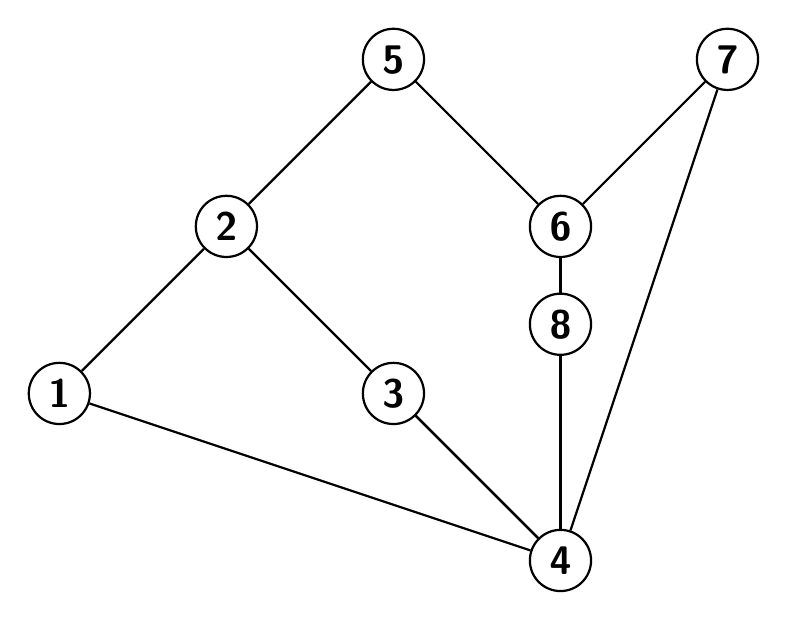
\begin{tikzpicture}[auto, node distance=3cm, every loop/.style={},
                    thick,main node/.style={circle,draw,font=\sffamily\Large\bfseries}]

  \node[main node] (1) {1};
  \node[main node] (2) [above right of=1] {2};
  \node[main node] (3) [below right of=2] {3};
  \node[main node] (4) [below right of=3] {4};
  \node[main node] (5) [above right of=2] {5};
  \node[main node] (6) [below right of=5] {6};
  \node[main node] (7) [above right of=6] {7};
  \node[main node] (8) [above of=4] {8};
        
  \path[every node/.style={font=\sffamily\small}]
    (1) edge node [left] {} (4)
    (2) edge node [right] {} (1)
        edge node [right] {} (5)
    (3) edge node {} (4)
        edge node [right] {} (2)
    (4) edge node [left] {} (3)
    (5) edge node {} (6)
    (6) edge node {} (8)
    (7) edge node {} (6)
        edge node {} (4)
    (8) edge node {} (4);
\end{tikzpicture}

The optimal solution for a vertex cover is $\{2,4,6\}$ with cardinality 3 so that OPT = 3.

LP solution would be to minimize  
$ X1 + X2 + X1 + X4 + X2 + X3 + X2 + X5 + X3 + X4 + X4 + X8 + X4 + X7 + X5 + X6 + X6 + X7 + X6 + X8 $ \\
subject to  \\

$ X1 + X2 \ge 1 $, 
$ X1 + X4 \ge 1 $, 
$ X2 + X3 \ge 1 $, 
$ X2 + X5 \ge 1 $, 
$ X3 + X4 \ge 1 $, 
$ X4 + X8 \ge 1 $, 
$ X4 + X7 \ge 1 $, 
$ X5 + X6 \ge 1 $, 
$ X6 + X7 \ge 1 $, 
$ X6 + X8 \ge 1 $, 
$ X1 \ge 0 $, 
$ -X1 \ge -1 $, 
$ X2 \ge 0 $, 
$ -X2 \ge -1 $, 
.
.
.
$ X8 \ge 0 $, 
$ -X8 \ge -1 $.

The problem can be written in matrix form as

$ Y * X \ge Z $

where Y is the solution vector.

Using a numerical software package, instead of maximizing an equation e.g. z = x + 2y, we can minimize its negative instead (-z = -x - 2y).
Instead of having the greater than or equal to sign, we can multiply the inequality by -1 and get the opposite less than or equal to sign ($ -X7 \le -1 $) using the linprog module from Python's scipy package.

\begin{minipage}{\linewidth}% Following stays together
\begin{lstlisting}[language=Python]
from scipy.optimize import linprog
obj = [1, 1, 1, 1, 1, 1, 1, 1]
lhs_ineq = [
	[ -1, -1, 0, 0, 0, 0, 0, 0],
	[ -1, 0, 0, -1, 0, 0, 0, 0],
	[ 0, -1, -1, 0, 0, 0, 0, 0],
	[ 0, -1, 0, 0, -1, 0, 0, 0],
	[ 0, 0, -1, -1, 0, 0, 0, 0],
	[ 0, 0, 0, -1, 0, 0, 0, -1],
	[ 0, 0, 0, -1, 0, 0, -1, 0],
	[ 0, 0, 0, 0, -1, -1, 0, 0],
	[ 0, 0, 0, 0, 0, -1, -1, 0],
	[ 0, 0, 0, 0, 0, -1, 0, -1]]
rhs_ineq = [-1, -1, -1, -1, -1, -1, -1, -1, -1, -1]
bnd = [
	(0, float("inf")),
	(0, float("inf")),
	(0, float("inf")),
	(0, float("inf")),
	(0, float("inf")),
	(0, float("inf")),
	(0, float("inf")),
	(0, float("inf"))] 
opt = linprog(c=obj, A_ub=lhs_ineq, b_ub=rhs_ineq, 
	bounds=bnd, method="revised simplex")
print(opt)
\end{lstlisting}
\end{minipage}



Running the above program generates on output array which is equal to the optimal:
\begin{lstlisting}[language=Python]
    x: array([0., 1., 0., 1., 0., 1., 0., 0.])
\end{lstlisting}





The rounded solution gives $\{2,3,4,5,6,7\}$ which has cardinality 6 so that the cost is 6.

(b) Consider the graph with vertices $V : \{1,2,3,4,5\} $ 

and edges $E : \{(1,2),(1,3),(1,5),(2,3),(2,5),(4,5)\} $. 

\begin{tikzpicture}[auto, node distance=3cm, every loop/.style={},
                    thick,main node/.style={circle,draw,font=\sffamily\Large\bfseries}]

  \node[main node] (1) {1};
  \node[main node] (2) [below right of=1] {2};
  \node[main node] (3) [below left of=2] {3};
  \node[main node] (4) [below left of=5] {4};
  \node[main node] (5) [below right of=4] {5};

        
  \path[every node/.style={font=\sffamily\small}]
    (1) edge node [left] {} (3)
        edge node [right] {} (5)
        edge node [right] {} (2)
    (2) edge node [right] {} (5)
        edge node [right] {} (3)

    (4) edge node [left] {} (5)
;
\end{tikzpicture}

We run a corresponding program to solve the LP problem for this graph.

\begin{minipage}{\linewidth}% Following stays together
\begin{lstlisting}[language=Python]
from scipy.optimize import linprog
obj = [1, 1, 1, 1, 1]
lhs_ineq = [
	[ -1, -1, 0, 0, 0],
	[ -1, 0, -1, 0, 0],
	[-1, 0, 0, 0, -1],
	[0, -1, 0, 0, -1],
	[0, -1, -1, 0, 0],
	[ 0, 0, 0, -1, -1]]
rhs_ineq = [-1, -1, -1, -1, -1, -1]
bnd = [
	(0, float("inf")),
	(0, float("inf")),
	(0, float("inf")),
	(0, float("inf")),
	(0, float("inf"))] 
opt = linprog(c=obj, A_ub=lhs_ineq, b_ub=rhs_ineq, 
	bounds=bnd, method="revised simplex")
print(opt)
\end{lstlisting}
\end{minipage}


Solving the LP problem gives the solution
\begin{lstlisting}[language=Python]
    x: array([0.5, 0.5, 0.5, 0.5, 0.5])
\end{lstlisting}


That means the cover should be the complete set of nodes and that is also the rounded solution.

But it is trivial to see that the set 2,3,5 is much cheaper and therefore the LP solution in this case differs in cost from the optimal solution.


\noindent \textbf{Alternative approaches}


In these cases we have looked at the properties of certain graphs that we chose beforehand. It could also be interesting to generate many random graphs and then checking the properties of the randoms graphs.

\end{problem}

\noindent
\hrulefill

\begin{problem}
 
\end{problem}


% \printbibliography %Prints bibliography
\end{document}

%%% Local Variables:
%%% mode: latex
%%% TeX-master: t
%%% End:
